% =====================================================================
%  FIGURE DOCUMENT -- submitted as its own file, separate from main.tex.
%  The journal asks that new submissions combine all figures into one
%  document, with each legend immediately following its figure.
%  Legends here are identical to the "Figure Legends" section of main.tex.
%
%  All three figures are anonymous: no institution, no repository, no filenames
%  that identify the authors.
%
%  Figures 1 and 3 are built by paper/tex/make_figures.py and copied in.
%  Figure 2 is built by make_rsna_figures.py in this directory.
%  Figures are numbered in order of first citation in main.tex.
%
%  Build: tectonic figures.tex
% =====================================================================
\documentclass[11pt,letterpaper]{article}

\usepackage[T1]{fontenc}
\usepackage[utf8]{inputenc}
\usepackage{mathptmx}
\usepackage[margin=1in]{geometry}
\usepackage{graphicx}
\usepackage{siunitx}

\sisetup{group-separator={,},group-minimum-digits=4}
\pagestyle{empty}
\setlength{\parindent}{0pt}
\setlength{\parskip}{0.6em}

\begin{document}

\begin{center}

\includegraphics[width=\textwidth]{figures/fig1_collapse.pdf}
\end{center}

\textbf{Figure 1.} One pixel-blind score vector, read at two units, on the RSNA
2019 Intracranial Hemorrhage benchmark (\num{752802} slices, \num{21744}
series, \num{18938} patients). \textbf{(A)} Slice-level area under the receiver
operating characteristic curve (AUC) joined to patient-level AUC for each of
the six official labels, with 95\% subject-clustered bootstrap intervals and
the within-series label permutation null at the patient unit. Nothing changes
between the two readings of a pair except the unit at which the ranking is
performed; every patient-level point estimate lies below chance, and four of
the six intervals lie wholly below it, the epidural and intraventricular
intervals crossing 0.5. \textbf{(B)} Width of the correct subject-clustered
interval divided by the width of the naive slice-resampled interval on the same
six labels: the naive interval is 1.51 to 1.99 times too narrow.

\clearpage

\begin{center}
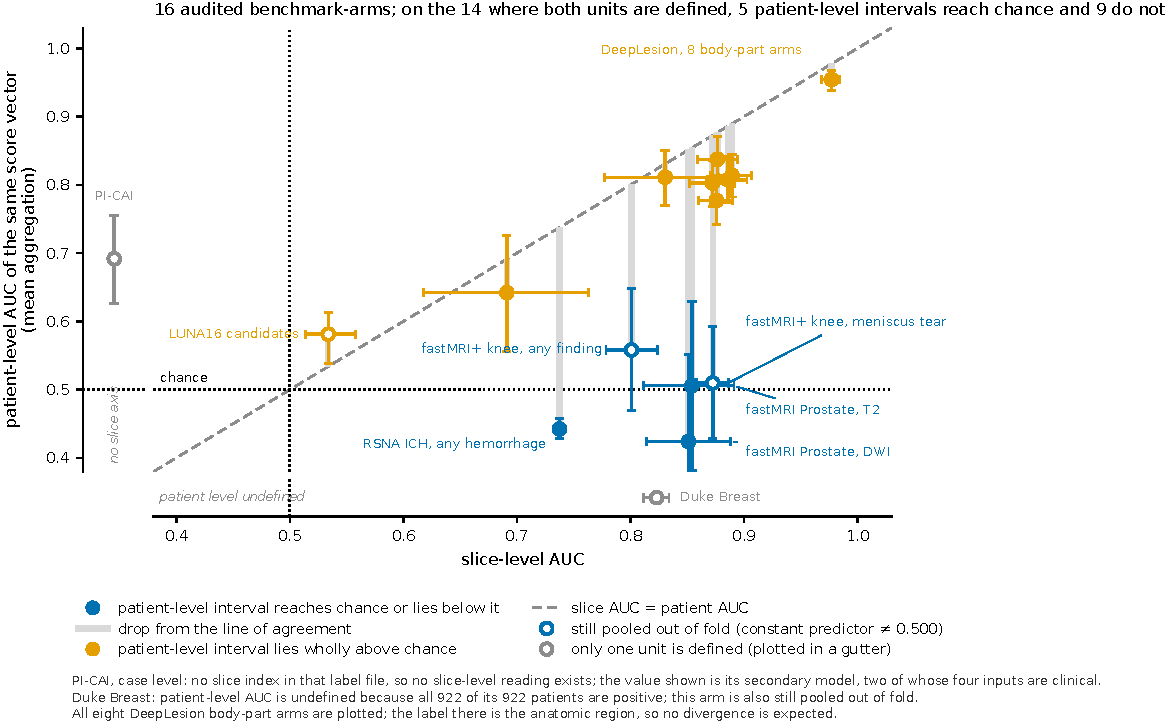
\includegraphics[width=\textwidth]{figures/fig2_unit_scatter.pdf}
\end{center}

\textbf{Figure 2.} The same pixel-blind score vector read at two units, for
every audited benchmark-arm. Each point is one arm: its slice-level area under
the receiver operating characteristic curve (AUC) against the patient-level AUC
of the identical score vector after mean aggregation, with 95\%
subject-clustered bootstrap intervals on both axes. The dashed diagonal is the
line on which the two units agree, and the grey stem below each point is the
distance that arm falls from it. Of the seven arms for which both units are
defined, five have a patient-level interval that reaches chance or lies below
it; the two that do not are DeepLesion, whose labels are anatomic regions that
relative slice position predicts at either unit, and LUNA16, which moves little
at either. Values are for the 20-bin positional baseline except PI-CAI, whose
positional baseline is exactly 0.500 and whose strongest zero-image baseline is
an acquisition-metadata tree. The two arms defined at only one unit are drawn in
the margins rather than in the field, so that a value that does not exist cannot
be read as a low one: PI-CAI's label file carries no slice index, and Duke
Breast's patient-level AUC is undefined because all 922 of its 922 patients are
positive.

\clearpage

\begin{center}
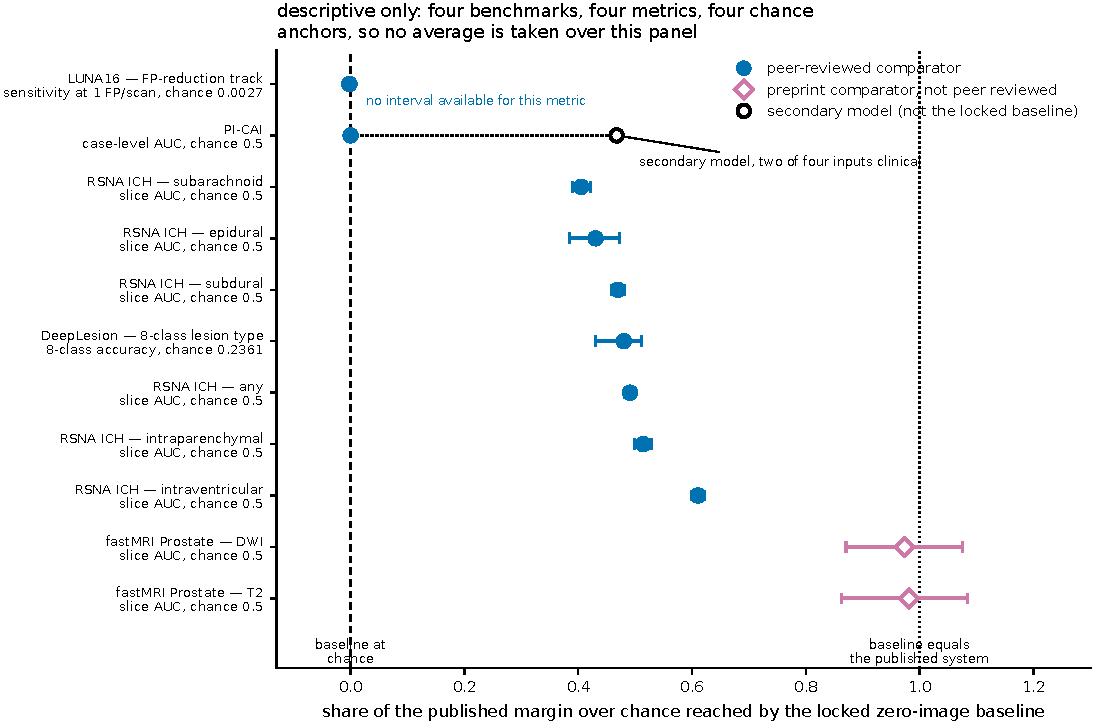
\includegraphics[width=\textwidth]{figures/fig3_trivial_fraction.pdf}
\end{center}

\textbf{Figure 3.} Trivial fraction---the share of a published margin over
chance reached by a pixel-blind model---for the strongest published comparator
per benchmark-arm. Peer-reviewed median 0.469, IQR 0.437 to 0.490 ($n=9$); the
shaded band is that IQR, and error bars are 95\% subject-clustered bootstrap
intervals propagating uncertainty in the baseline only. Rows whose comparator
is a preprint that has not been peer reviewed are marked as such; they are the
two highest here, at 0.973 and 0.981, and no row in this figure reaches 1.
LUNA16 is plotted at $-0.002$, computed on sensitivity at one false positive per
scan---one operating point of the challenge's own competition performance
metric, against a random-score reference of 0.0027 rather than against 0.5---for
which no interval is available. The open circle on the PI-CAI row marks its
positional baseline alone, which is exactly 0.500 area under the curve---the
correct registration of ``inapplicable,'' because that label file has no slice
index---while the filled marker is its strongest zero-image baseline, over
acquisition metadata.

\end{document}
